\subsection{3D Gaussian Splatting}

NeRF дает отличную базу к представлению сцен в виде полей излучения, однако представлять их в виде нейросети очень дорого: рендер, а следовательно и обучение, требуют обращаться к MLP миллионы раз (в оригинальной статье предлагается делать в общей сумме 256 сэмплов на каждом луче, при разрешении изображения 800 на 800 пикселей потребуется определить цвет для 640 тысяч лучей). Из-за этого рендер каждов может занимать минуты, а обучение --- дни.

Можно пробовать дорабатывать оригинальную идею чтобы сократить количество сэмплов или размер нейросети, как например делают в работе \cite{M_ller_2022}. Но в данный момент самым обсуждаемым решением оказывается отказ от неявного представления в пользу явного. Основоположником этого подхода стала работа \cite{kerbl3Dgaussians}, предложившая размещать в трехмерном пространстве гауссианы.

Подход аналогичен рассматриваемому в разделе \ref{sec:raycasting_splatting} методу Splatting, где ядром выступает распределение Гаусса с центром $\mu$ (матожиданием) и формой $\Sigma$ (матрицей ковариации). Задаются гауссианы следующим образом
%
\[
	G(\mathbf x) = e^{-\frac12 (\mathbf x-\mu)^t \Sigma^{-1} (\mathbf x - \mu)}.
\]
%
Полем излучения гауссианы делает то, что каждой гауссиане помимо её прозрачности $\alpha$ также сопоставляется зависимый от взгляда цвет: с помощью сферических гармоник.

Сферические гармоники --- это базис комплекснозначных функций, которые сводятся к базису вещественнозначных, на сфере по аналогии с рядом фурье на числовой прямой. Так как направление взгляда $\mathbf d$ отождествляется со сферой $S^2$, то сферические гармоники оказываются удобным аппаратом запекания с их помощью зависимого от взгляда цвета. 

Базисная функция обозначается как $Y_{lm}$, где $l$ --- её степень (соответствует уровню детализации), а $m$ --- порядок (ориентация). На рисунке \ref{fig:spherical_functions} изображены некоторые из таких функций.

\begin{figure}[ht]
	\centering
	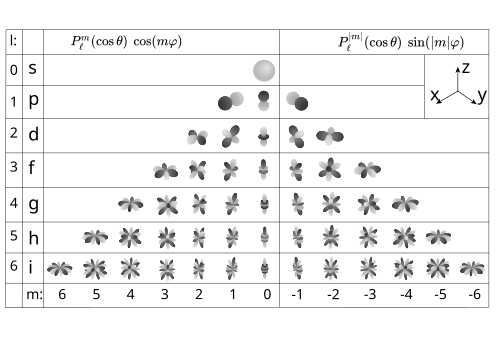
\includegraphics[width=\textwidth]{assets/Sphericalfunctions.png}
	\caption{Некоторые сферические гармоники. Белым здесь показаны числа больше нуля, черным - меньше нуля. Удаление от центра соответствует абсолютной величине.}
	\label{fig:spherical_functions}
\end{figure}

Тогда насыщенность каждого канала по направлению взгляда может быть закодировано как разложение по этому базису:
%
\[
	C(\mathbf d) = \sum_{l=0}^N \sum_{m=-l}^l c_{lm} Y_{lm}(\mathbf d),
\]
%
который удобно записать отождествить с вектором $\mathrm{sh} = (c_{0,0}, c_{1,-1}, \dots, c_{N, N})$.

Следующий вопрос, требующий рассмотрения --- это построение изображения. Если имеется гауссиана с уже вычисленным цветом и известными $\mu$, $\Sigma$, надо уметь строить её изображение на экране. Этот процесс раскрыт в работе \cite{zwicker2001ewa}.

Первым этапом будет перевод гауссианы из её положения в мировых координатах в координаты камеры. Это абсолютно линейный процесс, и ему соответствует поворот $W$ и перенос $\mathbf c$
%
\[
	\mu_\text{cam} = W\mu + \mathbf c,
\]
%
а для матрицы ковариации (если обозначим за $X$ распределение которое соответствует этой гауссиане)
%
\[
	X_\text{cam} = WX + \mathbf c
\]
\[
	\Sigma_\text{cam} = E \left[
		(X_\text{cam} - \mu_\text{cam})
		(X_\text{cam} - \mu_\text{cam})^t
	\right] = W \Sigma W^t
\]
%
Далее потребуется переход в так называемое пространство лучей, интуиция за которым изображена на рисунке \ref{fig:camera_to_ray_space}. По нему видно, что этот переход нелинеен, но гауссианы в пространстве обычно небольшие, поэтому в рамках переноса одной можно воспользоваться приближением с помощью матрицы Якоби в центре гауссианы:
%
\[
	J = \frac{\mathrm d \mathbf x}{\mathrm d \mathbf t} (\mu_\text{cam}).
\]
%
\begin{figure}[ht]
	\centering
	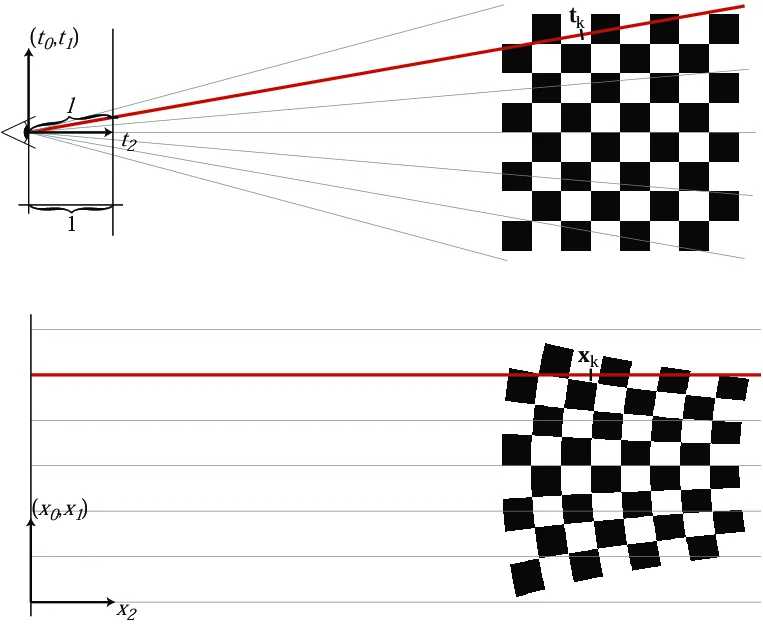
\includegraphics[width=\textwidth]{assets/camera_to_ray_space.png}
	\caption{Переход от координат $\mathbf t$ в пространство лучей $\mathbf x$.}
	\label{fig:camera_to_ray_space}
\end{figure}

Формула перехода имеет вид:
\[
	\begin{pmatrix} x_0 \\ x_1 \\ x_2 \end{pmatrix} =
	\begin{pmatrix}
		t_0 / t_2 \\
		t_1 / t_2 \\
		\| \mathbf t \|
	\end{pmatrix} =
	\begin{pmatrix}
		t_0 / t_2 \\
		t_1 / t_2 \\
		\sqrt{t_0^2 + t_1^2 + t_2^2}
	\end{pmatrix},
\]
%
а значит Якобиан вычисляется как
\[
	J = \begin{pmatrix}
		1 / t_2 & 0 & - t_0 / t_2^2 \\
		0 & 1 / t_2 & - t_1 / t_2^2 \\
		t_0 / \| \mathbf t \| & t_1 / \| \mathbf t \| & t_2 / \| \mathbf t \|
	\end{pmatrix}.
\]
%
Теперь его можно использовать, чтобы отобразить гауссиану в пространство лучей по формуле
%
\[
	X' = J(X_\text{cam} - \mu_\text{cam}) + \mu', \quad \mu' = E[X']
\]
\[
	\Sigma' = E \left[
		(X' - \mu') (X' - \mu')^t
	\right] = J \Sigma_\text{cam} J^t.
\]
%
Далее, отпечаток этой гауссианы уже по ортогональной проекции может быть получен по ранее обсуждавшейся формуле маргинализации
%
\[
	G_\text{footprint}(x_0, x_1) = \int_{-\infty}^{+\infty} G'(\mathbf x) \mathrm dx_2,
\]
%
что известно также будет распределением Гаусса. Пусть матрица ковариации гауссианы $G'$ имеет вид
%
\[
	\begin{pmatrix}
		a & b & c \\
		b & d & e \\
		c & e & f
	\end{pmatrix}.
\]
%
Если обратить внимание, что маргинализация по $x_2$ есть в точности плотность распределения следующих случайных величин:
%
\[
	PX' =
	\begin{pmatrix}
		1 & 0 & 0 \\
		0 & 1 & 0
	\end{pmatrix}
	\begin{pmatrix} X'_1 \\ X'_2 \\ X'_3\end{pmatrix} =
	\begin{pmatrix} X'_1 \\ X'_2 \end{pmatrix},
\]
%
откуда можно посчитать матрицу ковариации отпечатка
%
\begin{multline*}
	\Sigma_\text{footprint} = E \left[
		(PX' - E[PX']) (PX' - E[PX'])^t
	\right] = \\ 
	= P E \left[
		(X' - EX') (X' - EX')^t
	\right] P^t = P \Sigma' P^t = \begin{pmatrix}
		a & b \\
		b & d
	\end{pmatrix}.
\end{multline*}
%
Таким образом получено, что матрица ковариации проекции (отпечатка) гауссианы $G$ может получена выкидываением третьей строки и третьего столбца из матрицы ковариации
%
\[
	\Sigma' = JW \Sigma W^t J^t.
\]
%
Последний оставшийся вопрос --- их обучение. Оно осуществляется градиентным спуском по ошибке рендера $\hat I \in \mathbb R^{W \times H \times 3}$ в сравнении с целевым изображением $I \in \mathbb R^{W \times H \times 3}$. В оригинале предлагается использовать комбинацию следующих ошибок:
\[
	\mathcal L_1 = \frac{1}{WH \cdot 3} \sum | \hat C_i - C_i |,
\]
\[
	\mathcal L_\text{D-SSIM} = \frac{1 - \mathrm{SSIM}}{2}, \quad \mathrm{SSIM} = \frac{
		(2 \mu_1 \mu_2 + c_1) (\sigma_{12} + c_2)  
	}{
		(\mu_1^2 + \mu_2^2 + c_1) (\sigma_1^2 + \sigma_2^2 + c_2)
	},
\]
%
где $\mu_1, \mu_2, \sigma_1, \sigma_2$ --- среднее и дисперсия $\hat I$ и $I$ соответственно, $\sigma_{12}=\mathrm{cov} (\hat I, I)$.

Для того, чтобы можно было сделать по ним градиентный спуск, рендер $\hat I$ должен быть дифференцируемым. Нетрудно увидеть, что недифференцируемых операций в процессе построения отпечатка не было, следовательно, осталось определиться какие параметры надо оптимизировать.

По факту уже имеются все нужные формулы кроме одной. Однако оптимизация $\Sigma_i$ (для гауссианы $G_i$) напрямую --- странная задача, так как после каждого шага градиентного спуска придется контролировать, что матрица осталась симметричной положительно определенной, вместо этого предлагается рассмотреть геометрическую интуицию: $\Sigma_i$ отвечает за растяжение и поворот гауссианы, а значит представима в виде
%
\[
	\Sigma_i = E \left[
		(RSX - E[RSX]) (RSX - E[RSX])^t
	\right] = RSS^tR^t,
\]
%
где
%
\[
	S = \mathrm{diag} (s_x, s_y, s_z), \quad R^t=R^{-1}.
\]
%
$(s_x, s_y, s_z) = s$ уже можно оптимизировать напрямую, а матрица $R$ (поворот) содержит в себе излишне много ненулевых элементов, следить за её ортогональностью также тяжело, зато известно, что поворот в трехмерном пространстве на самом деле могут описывать $3$ числа, а также, что их описывают кватернионы длины $1$:
%
\[
	q = q_r + \mathbf i q_i + \mathbf j q_j + \mathbf k q_k, \quad
	q_r^2 + q_i^2 + q_j^2 + q_k^2 = 1.
\]
%
Из них можно сконструировать любую матрицу поворота которому они соответствуют по формуле
%
\[
	R(q) = \begin{pmatrix}
		1 - 2(q_j^2 + q_k^2) & 2(q_i q_j - q_r q_k) & 2(q_i q_k + q_r q_j) \\
		2(q_i q_j + q_r q_k) & 1 - 2(q_i^2 + q_k^2) & 2(q_j q_k - q_r q_i) \\
		2(q_i q_k - q_r q_j) & 2(q_j q_k + q_r q_i) & 1 - 2(q_i^2 + q_j^2)
	\end{pmatrix}.
\]
%
В процессе оптимизации потребуется контролировать только длину кватерниона.